\documentclass[a4paper,10pt,oneside]{scrartcl}

\usepackage[utf8]{inputenc}
\usepackage[a4paper]{geometry}
\usepackage{hyperref}
\usepackage{url}
\usepackage{color}
\usepackage{amsfonts}
\usepackage{graphicx}

\input{../hol_commands.inc}

\title{Exercise 4}

\begin{document}

\begin{center}
\usekomafont{sectioning}\usekomafont{part}ITP Exercise 4
\webversion{}{\\\small{due Wednesday 24th May}}
\end{center}
\bigskip


\section{Functional Arrays}

Arrays are not easily available in pure functional programs. However,
one can easily encode finite maps with natural numbers as keys. One
such finite map implementation is known as \emph{functional arrays}.
Functional arrays are binary trees that use the binary representation
of the key to determine the position in the tree. As a result, the
trees are always balanced. This is illustrated by the following picture:

\begin{center}
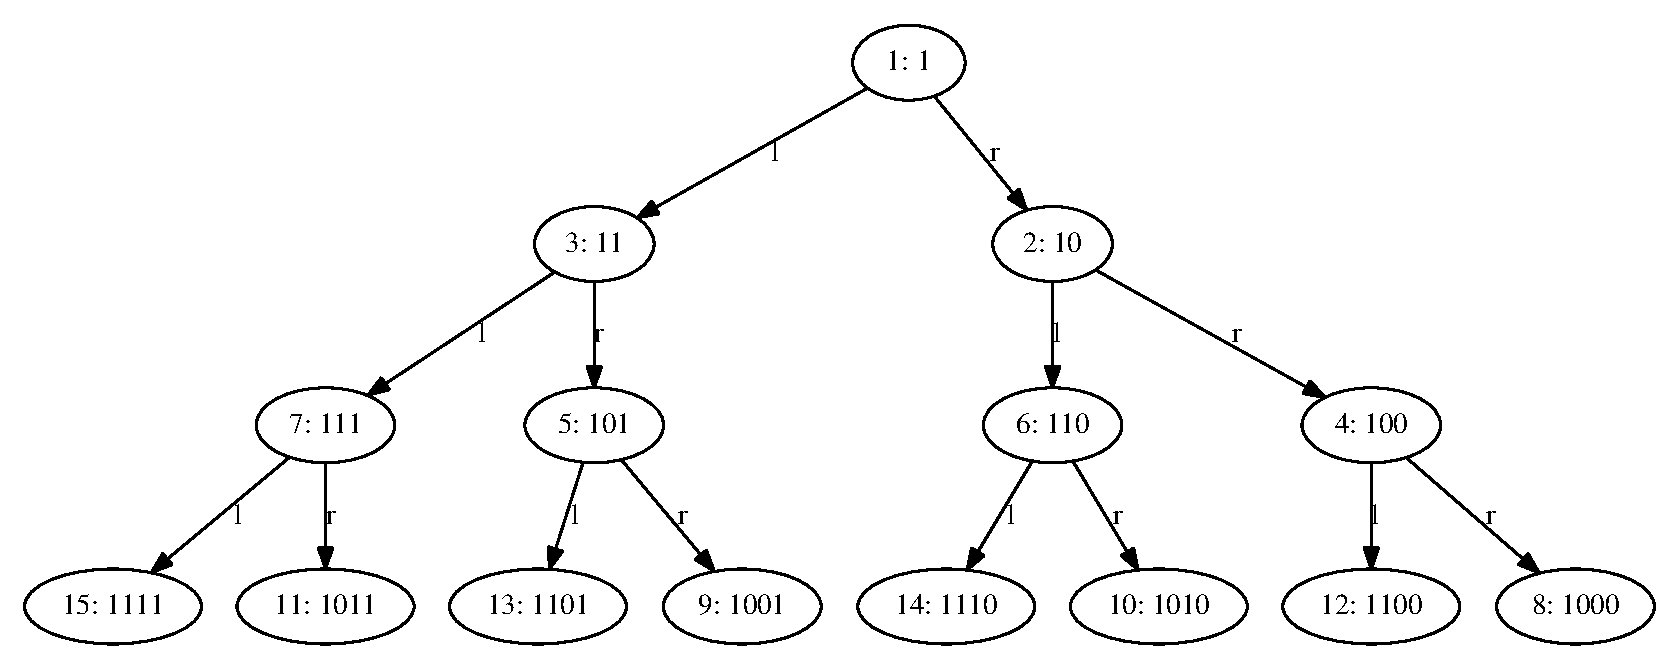
\includegraphics[width=14cm]{func_array.eps}
\end{center}

The nodes in this tree are annotated with the both the decimal and the binary representation of
their keys. The root node is for key 1, key 0 is not allowed. All values in 
the right subtree are even, all in the left odd. This means that the last digit is
always 0 or always 1. We then continue with this scheme recursively. At level 2 we look at the 
second bit, level 3 looks at the third bit and so on.

Navigating to the node for key $k$ can easily be implemented recursively. We check whether
$k$ is 1. If so, we look at the root node of our tree. Otherwise, we check whether $k$ is even.
If it is, we search for key $k\ \textit{DIV}\ 2$ in the right subtree, otherwise we look for
$k\ \textit{DIV}\ 2$ in the left subtree. Another way of describing the procedure is that we
always look at the last bit. If we see 0, we go to the right subtree, if we see 1 we go to the left subtree. We then throw the last bit away and continue. Once we reach the number 1, we stop.

\bigskip

Let's implement functional arrays in HOL. Please use the file
\texttt{e4\_arraysScript.sml} for this purpose. It contains auxiliary
definitions and some outline. Please read all of the exercise sheet
(except perhaps the hints section) before you start working.


\subsection{Datatype}

Define a datatype for functional arrays. This should be a binary tree type with leafs and nodes.
Leafs don't store any information. Each node should have a left and a right subtree as well as perhaps a value. Some keys might have a value stored, other not. So, please use an option type here.

In C one would have nodes with a left- and right subtree pointer. NULL values in these pointers would indicate that we don't have a subtree. This role of NULL pointers is in our functional implementation taken by leafs. Notice that leafs are not shown in the picture above. Each node in the last row above has implicitly a left and a right subtree, which are leafs. 


\subsection{Implement Basic Operations}

Let's now implement a lookup, an update, a remove operation as well as a constant for empty arrays.
Checking the bits of the key directly in the recursive definitions of these operations is fiddly.
One has to reason about arithmetic a lot and deal with some awkward termination conditions.
Therefore, I took already care for you of this fiddly part. The function \hol{num2arrayIndex} takes
a key and returns an array index. An array index is encoded as a list of booleans. If the list is empty, we should stop at the current node. If it starts with \texttt{F} we should look at the left subtree, if it is \texttt{T} at the right one. There is also an inverse operation \hol{arrayIndex2num} as well as a few lemmata. Notice, that \hol{num2arrayIndex} adds implicitly 1 to the number before
looking at the bits. Thus, we can handle 0 and don't need a special case.

\subsubsection{\texttt{EMPTY\_ARRAY}}

Define a constant \texttt{EMPTY\_ARRAY} that represents an array, which has no values stored in it at all.


\subsubsection{\texttt{UPDATE} and \texttt{REMOVE}}

Define an update function. Start with defining a function \texttt{IUPDATE v a idx} that updates array \texttt{a} to contain \texttt{v} for index \texttt{idx}. It should return the updated array. Then use the definition of \texttt{UPDATE} already present in the theory to lift this definition to keys that are natural numbers.
Similarish define a function \texttt{REMOVE a idx} that removes the value stored for index \texttt{idx} from array \texttt{a}. No value should be stored for this index in the resulting array. 

The remove and update functions are very similar. It is beneficial to define a generalised update function that takes an optional value argument. If a value is provided, the current value is updated with it. If no value is provided, the current one is removed.

\subsection{Test your definition}

Use \texttt{EVAL} to test whether your definitions work as expected.


\subsection{Visualise Trees}

To install HOL, you needed to install the graphviz tool 
(\url{http://www.graphviz.org/}). Let's use this tool to visualise your trees.
I already coded an auxiliary library to communicate with graphviz. You need to
write syntax functions for your array type. I recommend having a look at the implementation
of an existing syntax library like \texttt{optionSyntax}. Then code functions

\begin{itemize}
\item \texttt{is\_array\_leaf :\ term -> bool}
\item \texttt{is\_array\_node :\ term -> bool}
\item \texttt{dest\_array\_node :\ term -> (term * term option * term)}
\end{itemize}

Use the provided library \texttt{dot\_graphLib} to visualise your
arrays. Some example code is provided in
\texttt{e4\_arraysLib.sml}. Familiarise yourself with this code. The
example array \texttt{a2} should have for $n < 10$ the value $n$
stored at key $3*n$ all other keys have no value stored.  When you
visualise \texttt{a2} the result should look as follows:

\begin{center}
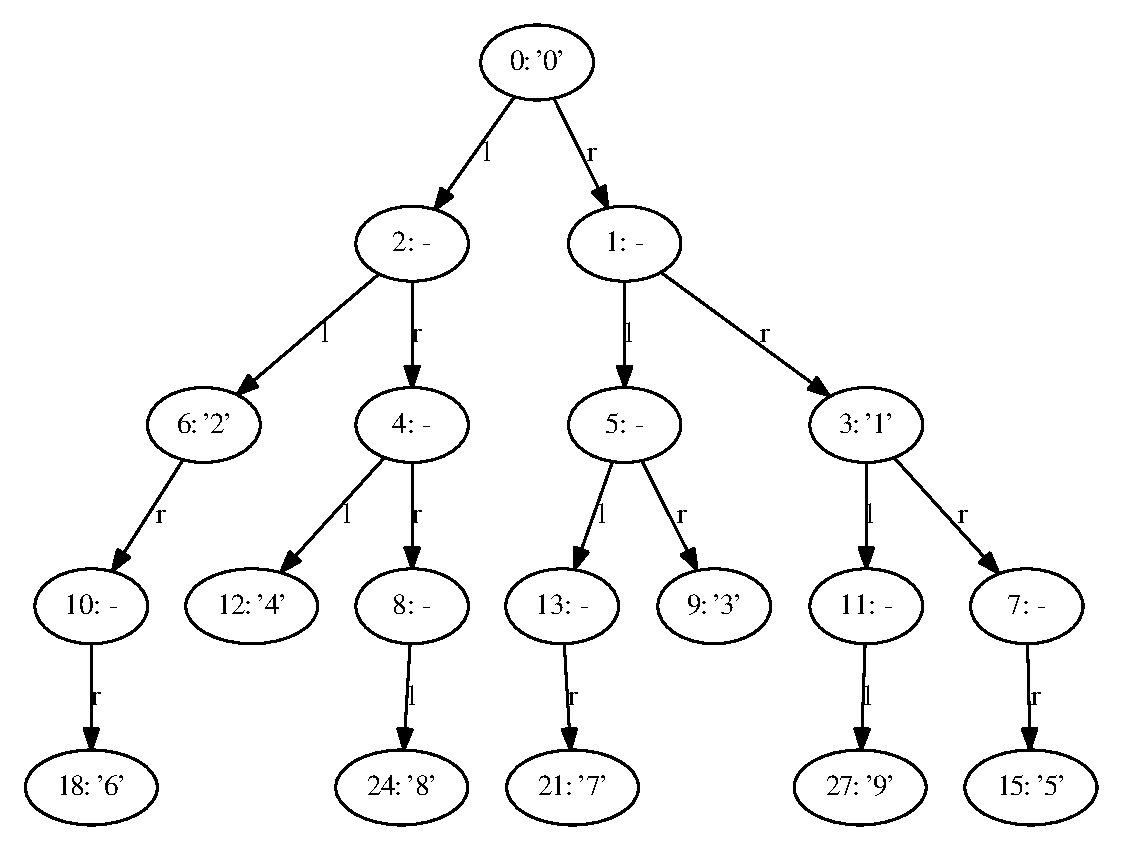
\includegraphics[width=14cm]{a2.eps}
\end{center}

This is a good test of whether your \texttt{UPDATE} works as expected. Feel free however, to
delay this exercise till after the proofs, if you prefer that.


\subsubsection{\texttt{LOOKUP}}

Define a lookup function. Similar to \texttt{UPDATE} define \texttt{ILOOKUP} on indexes first and
then lift it to numbers. \texttt{LOOKUP a k} should return \texttt{SOME v} iff value \texttt{v} is
stored for key \texttt{k} and \texttt{NONE} if no value is stored.


\subsection{Test your definition}

Use \texttt{EVAL} to test whether your definition of \texttt{LOOKUP} works as expected.


\subsection{Basic Properties}

Show that you indeed implemented a finite map datastructure. For this purpose fill in the missing
proofs in \texttt{e4\_arraysScript.sml}. Make sure that the resulting theory compiles and can be loaded by \texttt{e4\_arraysLib.sml}.

You should prove the following properties:

\begin{enumerate}
\item \texttt{!k.\ LOOKUP EMPTY\_ARRAY k = NONE}
\item \texttt{!v n n' a.\ LOOKUP (UPDATE v a n) n' =\\
\-\qquad (if (n = n') then SOME v else LOOKUP a n')}
\item \texttt{!n n' a.\ LOOKUP (REMOVE a n) n' = (if (n = n') then NONE else LOOKUP a n')}
\item \texttt{!v1 v2 n a.\ UPDATE v1 (UPDATE v2 a n) n = UPDATE v1 a n}
\item \texttt{!v n a.\ UPDATE v (REMOVE a n) n = UPDATE v a n}
\item \texttt{!v n a.\ REMOVE (UPDATE v a n) n = REMOVE a n}
\item \texttt{!v1 v2 a n1 n2.\ n1 <> n2 ==>\\\-\qquad
     ((UPDATE v1 (UPDATE v2 a n2) n1) = (UPDATE v2 (UPDATE v1 a n1) n2))}
 \item \texttt{!v a n1 n2.\ n1 <> n2 ==>\\\-\qquad
     ((UPDATE v (REMOVE a n2) n1) = (REMOVE (UPDATE v a n1) n2))}
 \item \texttt{!a n1 n2.\ n1 <> n2 ==>\\\-\qquad
     ((REMOVE (REMOVE a n2) n1) = (REMOVE (REMOVE a n1) n2))}
\end{enumerate}

\section{Hints}

If you perform your proofs naively, you need a lot of case-splits and everything gets
very lengthy. It is beneficial to use many auxiliary definitions and use them and many tiny
lemmata about them to avoid case-splits. It might for example be beneficial to introduce auxiliary
functions \texttt{VAL\_OF\_ROOT} and \texttt{GEN\_GET\_SUBARRAY} and derive the following properties:
\begin{itemize}
\item \texttt{!a. ILOOKUP a [] = VAL\_OF\_ROOT a}
\item \texttt{!a i idx.\ ILOOKUP a (i::idx) = ILOOKUP (GEN\_GET\_SUBARRAY i a) idx}
\end{itemize}




\end{document}

%%% Local Variables:
%%% mode: latex
%%% TeX-master: t
%%% End:
